\documentclass{beamer}
\usepackage{ dsfont }
\usepackage[utf8]{inputenc}
\usepackage[english]{babel}
\setbeamersize{text margin left=10pt, text margin right=10pt} %new code
\usepackage{graphicx}
\usepackage{float}
\usepackage{subcaption}
\usefonttheme{professionalfonts} % using non standard fonts for beamer
\setbeamerfont{frametitle}{series=\bfseries}
\usepackage{animate}
\usepackage{movie15}
\usepackage{breqn, bm}
\usepackage{amsmath}
\usepackage[skins]{tcolorbox}
\usepackage{subcaption}

\definecolor{notgreen}{RGB}{255,127,0}
\definecolor{green}{RGB}{49,150,3}
\setbeamerfont{headline}{size=\small}


%----------------------------------------------------------------------------------------
%	 Package
%----------------------------------------------------------------------------------------
\usepackage{color}
\usepackage{url}
\beamertemplatenavigationsymbolsempty
\definecolor{cadmiumred}{rgb}{0.8, 0.8, 0.8}

%----------------------------------------------------------------------------------------
%	 Presentation settings
%----------------------------------------------------------------------------------------

\usetheme{default}
\usecolortheme{default}

\setbeamertemplate{itemize items}[triangle] 
\setbeamertemplate{enumerate items}[default]
 
\title[Variational Drop Out]{
	Talk with Christoph Lampert \\ 
	\vspace{1cm}
	\textbf{\textcolor{black}{Variational Deep Learning}}}

\author{Ashuha Arseniy$^{1, 2}$, Dmitriy Molchanov$^{1, 3}$}
\institute[Bayesgroup, MIPT, SkolTech]{
	Bayesian Research Group$^1$, MIPT$^2$, SkolTech$^3$\\
	
	\medskip
	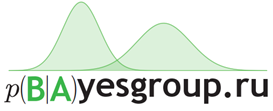
\includegraphics[scale=0.5]{./img/logo.png}
	
	\href{mailto:ars.ashuha@gmail.com}{\nolinkurl{ars.ashuha@gmail.com}}}

\date{\today}

\newcommand{\Expect}{\mathsf{E}}
\newcommand{\MExpect}{\mathsf{M}}
\newcommand{\cov}{\mathsf{cov}}
\setbeamertemplate{section in toc}[circle]

\addtobeamertemplate{navigation symbols}{}{%
	\usebeamerfont{footline}%
	\usebeamercolor[fg]{footline}%
	\hspace{1em}%
	\insertframenumber/\inserttotalframenumber
}


\begin{document}
\begin{frame}
	\titlepage 
\end{frame}

\begin{frame}{Two Stream of Machine Learning}
	\begin{columns}[T] % align columns
		\begin{column}{.5\textwidth}
						\vspace{-0.5cm}
						\begin{center}
							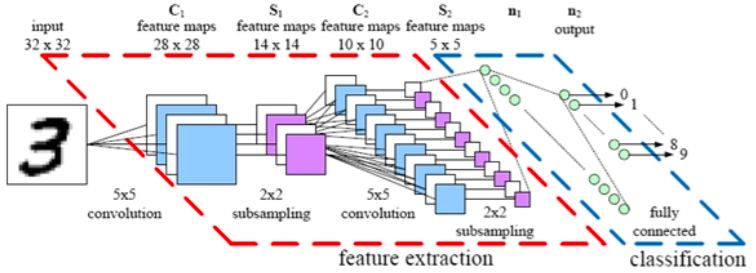
\includegraphics[scale=0.1]{./img/deepl.png}~~~\textbf{Deep Learning}
						\end{center}
						
						\vspace{-0.3cm}
			\begin{itemize}
				\item[\textcolor{green}{+}] \textcolor{green}{Rich non-linear models for classification and sequence prediction.}
				\item[\textcolor{green}{+}] \textcolor{green}{Scalable learning using stochastic approximations and conceptually simple.}
				\item[\textcolor{green}{+}] \textcolor{green}{ Easily composable with other gradient-based methods}
				\item[\textcolor{red}{$-$}] \textcolor{red}{Only point estimates}
				\item[\textcolor{red}{$-$}] \textcolor{red}{Hard to score models, do model selection and complexity penalisation.}
			\end{itemize}
		\end{column}
		\hfill%
		\hspace{-1cm}
		\begin{column}{.53\textwidth}
			\vspace{-0.5cm}
			\begin{center}
				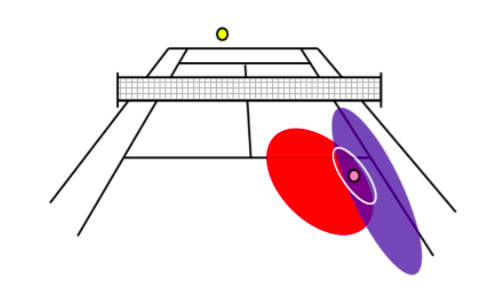
\includegraphics[scale=0.1]{./img/inf.png}~~~\textbf{Bayesian Reasoning}
			\end{center}

			\vspace{-0.3cm}
			\begin{itemize}
				\item[\textcolor{red}{$-$}] \textcolor{red}{ Mainly conjugate and linear models}
				\item[\textcolor{red}{$-$}] \textcolor{red}{Potentially intractable inference leading to expensive computation or long simulation times.}
					
				\item[\textcolor{green}{+}] \textcolor{green}{Unified framework for model building, inference, prediction and decision making}
				\item[\textcolor{green}{+}] \textcolor{green}{Explicit accounting for uncertainty and variability of outcomes}
				\item[\textcolor{green}{+}] \textcolor{green}{ Robust to overfitting; tools for model selection and composition.}
			\end{itemize}
		\end{column}%
	\end{columns}
\end{frame}

\section{Why it's a good idea?}

\begin{frame}{Review and Limitations of Deep Learning}	
	\begin{itemize}
		\item We all know well the linear models:
			$$\nu = \textbf{w}^t x + b, ~~p(y|x) = p(y|g(\nu); \theta)$$
			\begin{itemize}
				\item The basic function can be any linear function, e.g., affine, convolution
				\item $g(\cdot)$ is a function that we’ll refer to as an activation function
			\end{itemize}
		\item Recursive composition generalized linear functions give a Deep NN
			$$NuralNet(x) = g_n(W_n \cdot \dots \cdot g_1(W_1 \cdot x))$$
		\item While training we usually optimize Maximum Likelihood Estimation
	\end{itemize}

 	\begin{tcolorbox}[colback=black!80, colframe=black!80]
 		\begin{center}
 			\text{\textcolor{white}{A general framework for building non-linear, parametric models}}
 		\end{center}
 	\end{tcolorbox}
	
	\begin{center}
		\textcolor{red}{Problem: Overfitting of MLE leading to limited generalisation} 
	\end{center}
\end{frame}

\begin{frame}{Regularization of Deep Neural Nets}	

	
		\begin{columns}[T] % align columns
			\begin{column}{.8\textwidth}
				\vspace{-0.5cm}
	\begin{itemize}
		\item Regularization is essential to overcome overfitting
		\item A wide range of available regularization techniques:
		\begin{itemize}
			\item Large data sets
			\item Input noise and data augmentation
			\item L2 / L1 regularization
			\item Binary or Gaussian Dropout
			\item Batch normalization
		\end{itemize}
	\end{itemize}
			\end{column}
			\hfill%
			\hspace{-2.cm}
			\begin{column}{.53\textwidth}
				\vspace{-0.5cm}
				\begin{center}
					\vspace{.5cm}
					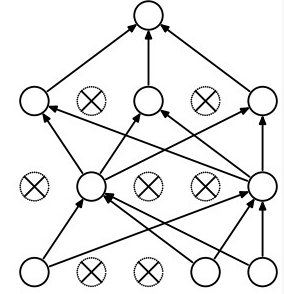
\includegraphics[scale=0.25]{./img/do.png}
				\end{center}
			\end{column}%
		\end{columns}
	
	\begin{tcolorbox}[enhanced,size=fbox,fontupper=\large\bfseries, colback=black!80, colframe=black!80]
		\begin{center}
			\text{\textcolor{white}{More robust loss function using MAP estimation instead}}
		\end{center}
	\end{tcolorbox}
	\vspace{0.2cm}
	\begin{columns}[T] % align columns
		\begin{column}{.7\textwidth}
			\vspace{-0.5cm}
			\begin{itemize}
				\item[\textcolor{green}{$+$}] Power of MAP estimators is that they provide some robustness to overfitting
				\item[\textcolor{green}{$+$}] Automatic determination of feature relevance
				\item[\textcolor{green}{$+$}] Can generate of frequentest confidence intervals
				\item[\textcolor{red}{$-$}] Creation of sensitivities to parametrization
			\end{itemize}
		\end{column}
		\hfill%
		\hspace{-1.2cm}
		\begin{column}{.53\textwidth}
			\vspace{-0.5cm}
			\begin{center}
				\vspace{-0.5cm}
				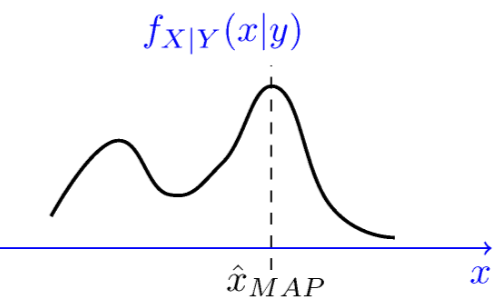
\includegraphics[scale=0.25]{./img/map.png}
			\end{center}
		\end{column}%
	\end{columns}
\end{frame}

\subsection{Review and Limitations of Bayesian Reasoning}
\begin{frame}{Review and Limitations of Bayesian Reasoning}
Our goal is to learn a model with weights $w$ of the $p(y|x, w)$
\vspace{0.2cm}

Let's use Bayesian  toolbox:
\begin{enumerate}
	\item We want to give posterior distribution $p(w|D) = p(w)p(D|w)/p(D)$
	\item But Bayes rule involves computationally intractable integrals 
	\item Therefore we will introduce parametric family $q_\phi(w)$
	\item Let's tune parameters such that $q_\phi(w)$ will be a close to $p(w|D)$
	\item Usually by maximize Variational Lower Bound		 

\end{enumerate}
$$\mathcal{L}(\phi) = \sum_{(x, y) \in D}\mathds{E}_{q_{\phi}} log~p(y|x, w) - D_{KL}(q_\phi(w), p_{prior}(w))$$
 
~~~~~~~~~~~~~~~~~~~~~~~~~~\textcolor{red}{likelihood expectation}~~~~~~~~~~~\textcolor{green}{regularizer}

 	\begin{tcolorbox}[enhanced,size=fbox,fontupper=\large\bfseries, colback=black!80, colframe=black!80]
 		\begin{center}
 			\text{\textcolor{white}{But, there is problem to apply this approach for Deep Nets}}
 		\end{center}
 	\end{tcolorbox}
 	
 	\begin{itemize}
 		\item $p(y|x, w)$ is Neural Net, so $\mathds{E}_{q_{\phi}} log~p(y|x, w)$ became intractable
	 	\item $\sum_{(x, y) \in D} \cdot$ contain sum over data, so EM-like algo cannot be applied
	\end{itemize}
\end{frame}



\section{How can we achieve this convergence?}

\subsection{Stochastic optimization}
\subsection{Approximate Bayesian Inference}
\begin{frame}{Approximate Bayesian Inference}
	The idea of stochastic optimization is quite simple, we will use:
	\begin{itemize}
		\item gradient based methods 
		\item unbiased gradient estimation instead of true gradient 
	\end{itemize} 
	\vspace{0.2cm}
	Can we apply this approach to optimize variational lower bound?
	$$\mathcal{L}(\phi) = \sum_{(x, y) \in D}\mathds{E}_{q_{\phi}} log~p(y|x, w) - D_{KL}(q_\phi(w), p_{prior}(w))$$
	\vspace{-0.7cm}
	\begin{enumerate}
		\item We can't take gradient by parameters by naive way.
		$$\nabla_\phi \mathds{E}_{q_{\phi}} log~p(y|x, w) \neq  \mathds{E}_{q_{\phi}} \nabla_\phi log~p(y|x, w) $$
		\item Let's use re-parametrization
		$$\nabla_\phi \mathds{E}_{q_{\phi}} log~p(y|x, w) = \mathds{E}_{N(\epsilon| 0, 1)} \nabla_\phi  log~p(y|x, w=f(\epsilon, \phi))$$
		\item For example $q_{\phi} = N(\phi_1, \phi_2^2)$ then $f(\epsilon, \phi) = \phi_1 + \phi_2 \cdot \epsilon$ 
		\item We can compute estimation of grad using double stochastic inference
	\end{enumerate}
\end{frame}

\begin{frame}{Variational Dropout}
	\begin{itemize}
		\item Affine layer with parameters matrix $W$ looks like
			$$B = A \cdot W$$
		\item Dropout is Bernoulli noise on input matrix and scaling 
			$$B = (A \odot (\xi / (1-p))) W~~~\xi \sim Bernoulli(p)$$
		\item Gaussian Noise with the same mean and variance works as well
			$$B = (A \odot \xi) W~~~\xi \sim Gaussian(1, p/(1-p)) = Gaussian(1, \alpha) $$
		\item It correspond to normal posterior distribution over weights 
			$$N(\mu, \sigma^2) = \mu + \sigma\cdot \epsilon,~~~\epsilon \sim Gaussian(1, \alpha)  $$
			$$B_{ij} = (A_i \odot \xi) W^j = \sum_t A_{it} \cdot (1 + \sqrt{\alpha}\cdot\epsilon) \cdot W_{tj} = $$
			$$ =  \sum_t N(A_{it}, \alpha A_{it}^2) \cdot W_{tj} = \sum_t A_{it}\cdot N(W_{tj}, \alpha W_{tj}^2) $$
		 $$q_{\alpha, \phi}(w_{ij}) = N(\phi_{ij}, \alpha\phi_{ij}^2)$$
	\end{itemize}
\end{frame}

\begin{frame}{Variational Dropout}
	During training neural net with dropout we optimize wrt $\phi$ with fixed $\alpha$
	$$\sum_{(x, y) \in D}\mathds{E}_{q_{\alpha, \phi}} log~p(y|x, w) \rightarrow \max_{\phi},~~~q_{\alpha, \phi}(w_{ij}) = N(\phi_{ij}, \alpha\phi_{ij}^2)$$
	
	With Log-uniform prior on $w_{ij}$
	
	\vspace{-0.3cm}
	$$p(log~|w_{ij}|) \propto c$$
	
	divergence does not depend on $\phi$
	
	\vspace{-0.3cm}
	$$- D_{KL}(q_{\alpha, \phi}(w_{ij}) || p(w_{ij})) = const + 0.5 \cdot log(a) + E_{\epsilon \sim N(1, \alpha)}log |\epsilon|$$
	
	Thus during dropout training we optimize variational lower bound w.r.t. $\phi$
	$$\sum_{(x, y) \in D}\mathds{E}_{q_{\alpha, \phi}} log~p(y|x, w) - D_{KL}(q_{\alpha, \phi}(w_{ij}) || p(w_{ij})) \rightarrow \max_{\phi}$$
	\begin{tcolorbox}[enhanced,size=fbox,fontupper=\large\bfseries, colback=black!80, colframe=black!80]
		\begin{center}
			\text{\textcolor{white}{Dropout is the special case of Bayesian Regularization}}
		\end{center}
	\end{tcolorbox}
	
	This is important because:
	\begin{enumerate}
		\item we can train personal alpha for weight, features or layer
		\item physical interpretation -- number of significant digits
	\end{enumerate} 
\end{frame}


\begin{frame}{Experiments Result}
	\begin{center}
		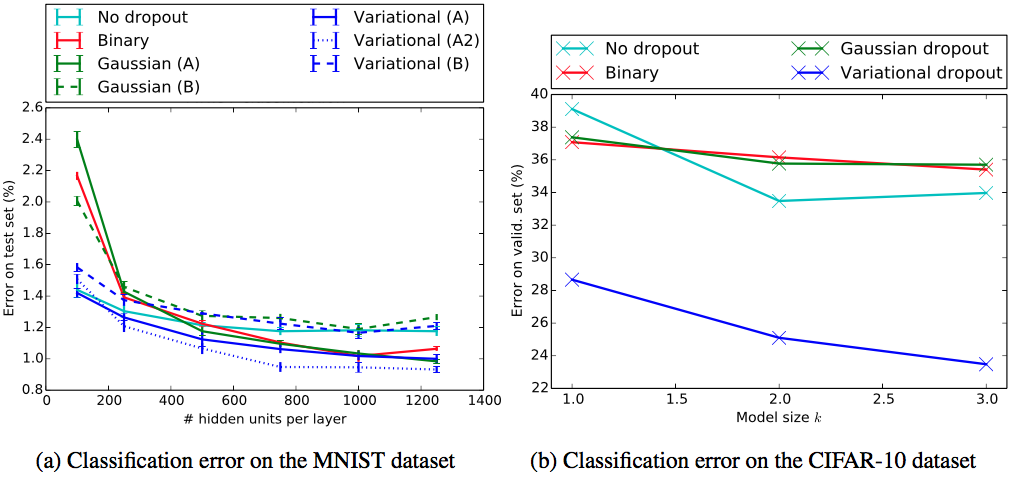
\includegraphics[scale=0.3]{./img/weling.png}
	\end{center}
	The experimental part of the paper was quite strange:
	\begin{enumerate}
		\item Alphas are clipped at 1: $\alpha < 1,~~p < 0.5$
		\item Training method for alphas and alpha sharing scheme are not
		specified
		\item The KL divergence was divided by 3 to prevent underfitting
	\end{enumerate}
\end{frame}

\begin{frame}{Our: ARD with VDO in Linear Models {\scriptsize[D. Molchanov]}}
	\begin{itemize}
		\item Relevance Vector Machine
		$$p(t|x, w) = \sigma(tw^tx)$$
		$$p(w|a) = N(w|0, diag(\alpha_1^{-1}, \dots, \alpha_n^{-1}))$$
		
		and determine $\alpha_i$ by optimizing evidence maximization
		
		$$P(X|\alpha) = \int p(t| x, w) p(w|\alpha) dw \rightarrow \max_{\alpha}$$
		
		if feature $j$ is irrelevant $\alpha_j \rightarrow +\infty, w_j \rightarrow 0$.
		\item Relevance Determination with Variational Drop Out
		$$\sum_{(x, y) \in D}\mathds{E}_{q_{\alpha, \phi}} log~\sigma(yw^tx) - D_{KL}(q_{\alpha, \phi}(w_{ij}) || p(w_{ij})) \rightarrow \max_{\phi}$$
		
		While we optimize Variational Lower Bound with log-Uniform Prior
		\begin{itemize}
			\item automatic relevance determination still exists
			\item tuning parameters of the prior distribution isn't necessary!!!
		\end{itemize}
	\end{itemize}
\end{frame}

\begin{frame}{Our: Divergence Estimation in VDO {\scriptsize[D. Molchanov]}}
	Approx. of the $D_{KL}$ which was obtained in the article is only true if  $\alpha < 1$
	\begin{center}
		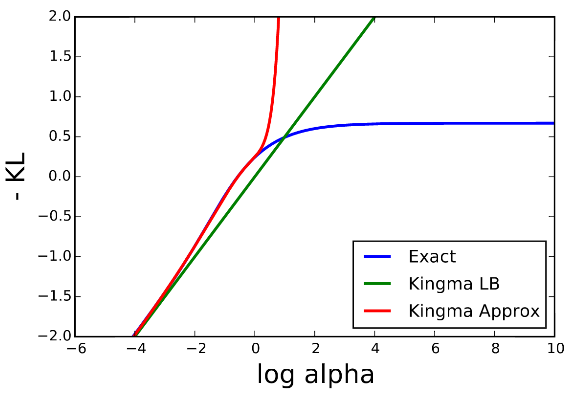
\includegraphics[scale=0.4]{./img/kl.png}
	\end{center}
	It was obtained by using sampling method.
		$$- D_{KL}(q_{\alpha, \phi}(w_{ij}) || p(w_{ij})) = const + 0.5 \cdot log(a) + E_{\epsilon \sim N(1, \alpha)}log |\epsilon|$$
\end{frame}

\begin{frame}{Our: ARD with VDO in Linear Models {\scriptsize[D. Molchanov]}}
	Synthetic data, 100000 objects, 10 relivant, 90 irrelivant features.
	\begin{itemize}
		\item Reliance determination (Regression, Classification)
			\begin{center}
				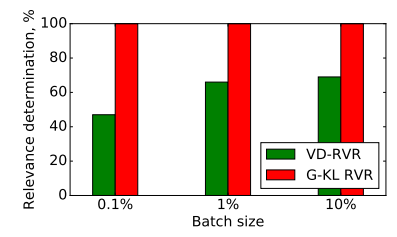
\includegraphics[scale=0.3]{./img/rdc.png}
				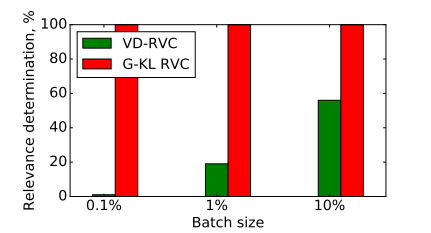
\includegraphics[scale=0.3]{./img/rdr.png}
			\end{center}
		\item Error Regression, Accuracy Classification
					\begin{center}
						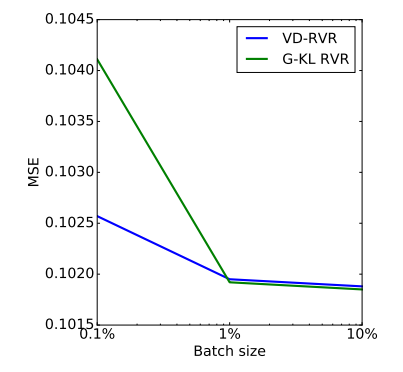
\includegraphics[scale=0.3]{./img/msec.png}
						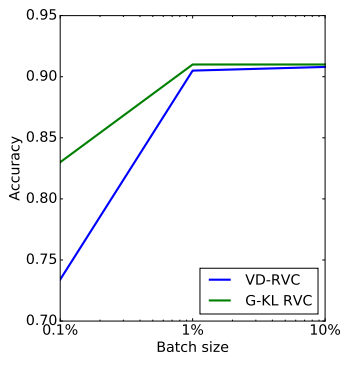
\includegraphics[scale=0.3]{./img/mser.png}
					\end{center}
	\end{itemize}
\end{frame}

\begin{frame}{Our: More Features {\scriptsize[D. Molchanov]}}
		\begin{center}
			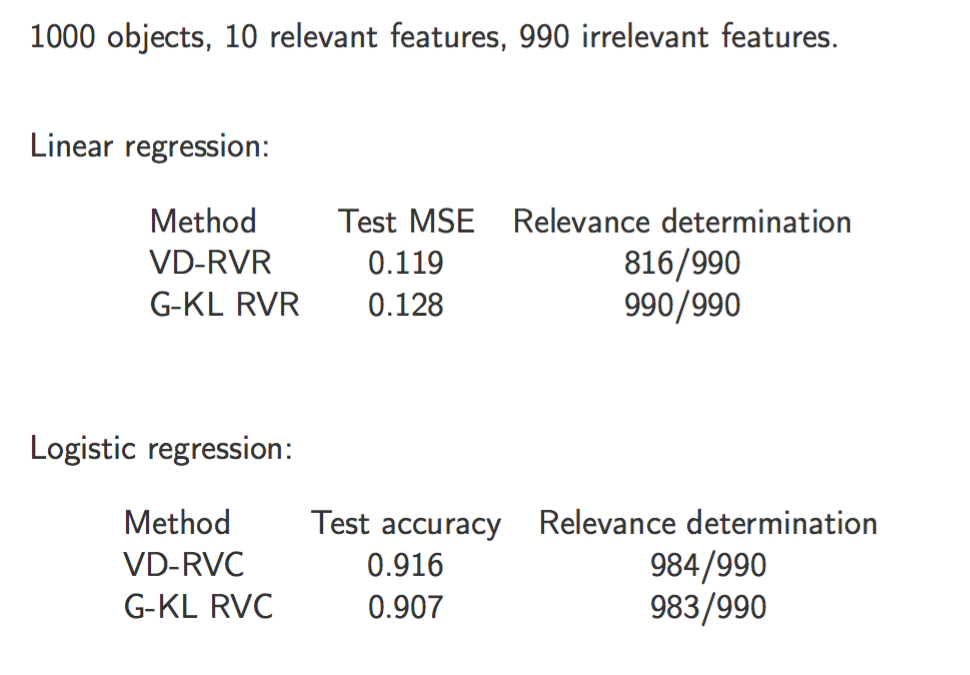
\includegraphics[scale=0.3]{./img/1000.png}
		\end{center}\end{frame}

\begin{frame}{Our: VDO picture classification without clipping}
	VDO picture classification without clipping
	\begin{center}
		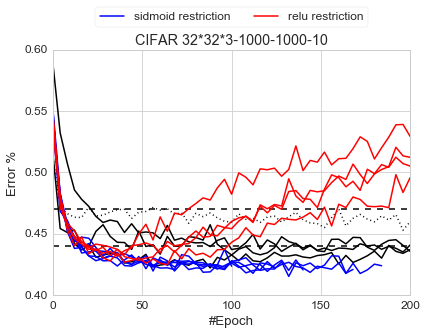
\includegraphics[scale=0.35]{./img/restr.png}
	\end{center}
	\vspace{-0.5cm}
	variance of gradients coursed faster over-fitting
		\begin{center}
			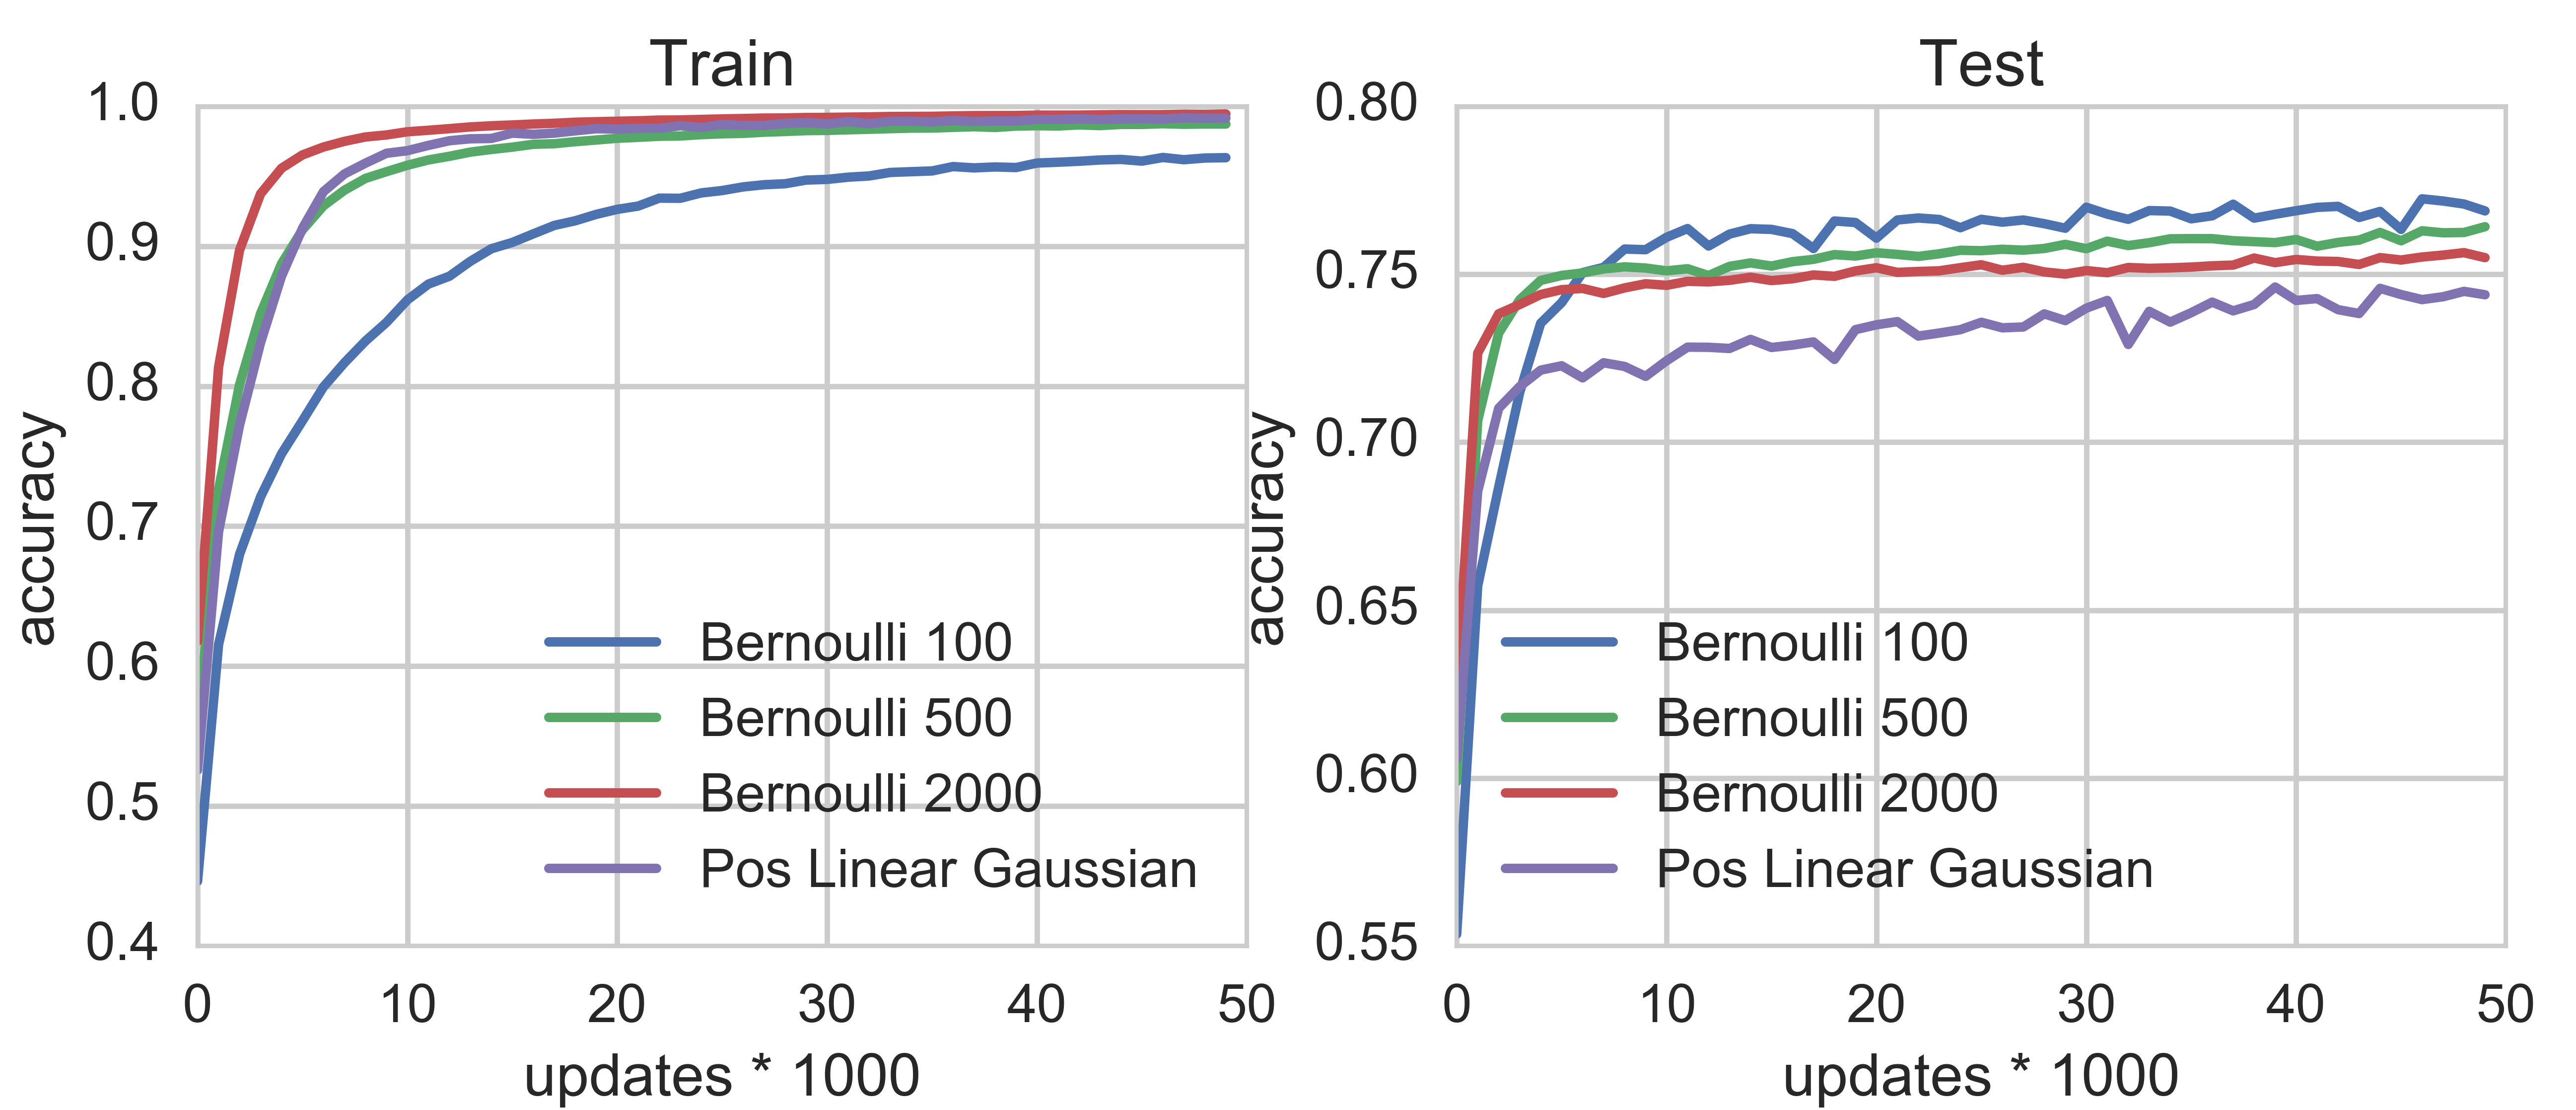
\includegraphics[scale=0.35]{./img/ove.png}
		\end{center}
\end{frame}

\begin{frame}{Our: future work}
	\begin{itemize}
		\item \textbf{Automatic Reliance determination}
			\begin{center}
				Determine personal alpha per layer/features with ARD
			\end{center}		
		\item \textbf{Incremental Learning}
		\begin{center}
			Using posterior distribution as a prior for next portion of data
		\end{center}		
		\item \textbf{Another regularization scheme}
		\begin{center}
			To use Log-Normal distribution to introduce unsymmetrical noise. 
		\end{center}	
	\end{itemize}
\end{frame}

\begin{frame}{References}

		\begin{thebibliography}{9}
			\setbeamertemplate{bibliography item}[book]
			\bibitem{A} Diederik P. Kingma, Tim Salimans, Max Welling: Variational Dropout and the Local Reparameterization Trick, \href{arxiv.org/abs/1506.02557}{arxiv.org/abs/1506.02557}
			\bibitem{B} Diederik P Kingma, Max Welling: Auto-Encoding Variational Bayes, \href{arxiv.org/abs/1312.6114}{arxiv.org/abs/1312.6114}
			\bibitem{C} Shakir Mohamed, http://shakirm.com/,  \href{http://blog.shakirm.com/wp-content/uploads/2015/10/Bayes_Deep.pdf}{http://blog.shakirm.com/wp-content/uploads/2015/10/Bayes_Deep.pdf}
		\end{thebibliography}
\end{frame}

\end{document}

